\chapter{Fixing ADD\_ADDR}
\label{chap:addaddr2}

\section{The ADD\_ADDR2 format}
There is an ongoing effort to move the current MPTCP specification from Experimental Track to Standard Track. Solving the ADD\_ADDR vulnerability is believed to be a fundamental step to reach the required security standards for the transition to happen.
By analyzing the nature of the vulnerability, various proposals have been elaborated to modify the design of the ADD\_ADDR option and they are reported in the official documentation for MPTCP security \cite{rfc7430}. The conceptual flaw behind the option is that no secret material related to the ongoing MPTCP is included in any of the fields. The only security mechanism performed on such message is the TCP-level sequence and acknowledge numbers, that an attacker has to know in order to inject such packets into an ongoing session.

A possible solution could be to add the receiver's token of the connection as a field in the ADD\_ADDR option. Such token is supposed to be unknown to the attacker that in turns would not be able to forge a valid ADD\_ADDR message. This solution wouldn't be effective if the attacker is able to eavesdrop the keys during the initial handshake, thus being able to retrieve the tokens for the connection as well; keys' eavesdrop is indeed a security concern related to MPTCP (see section \ref{keyseav}). It is not actually advisable to expose information regarding session's keys and tokens in clear inside the ADD\_ADDR option, since that would give more opportunities for eavesdropping.

Another possibility would be to maintain the ADD\_ADDR format unchanged but to block the attack at a later stage. A malicious ADD\_ADDR can be sent to trigger a SYN+MP\_JOIN generation at the client, but if the destination address of the SYN packet is added as part of the message used to calculate the HMAC value  for the MP\_JOIN messages, the attacker wouldn't be able to recompute the HMAC value after modifying the destination address. However, since addresses are not a stable piece of information in a network with NATs, using the destination address to calculate the HMAC is not a viable solution.

In order to achieve higher security levels maintaining NAT compatibility, a third option has been proposed. The idea is to add to the ADD\_ADDR option a new field containing the truncated HMAC value (rightmost 64 bits) calculated as follow: the key is the MPTCP key of the sender as originally agreed in the MP\_CAPABLE handshake; the message is the concatenation of the previous three fields in packet: address ID, advertised IP address, and port. The new format (figure \ref{fig:addaddr2}) has been formally specified for the first time in \rfc{6824bis-04} \cite{rfc6824bis04}, but slight modifications have been proposed and introduced in the newer version \rfc{6824bis-05} \cite{rfc6824bis05}, as explained in the following sections. For our analysis in this section and for the patches produced during the thesis work, the reference specification is \rfc{6824bis-04}.

\begin{figure}[!htb]
\centering
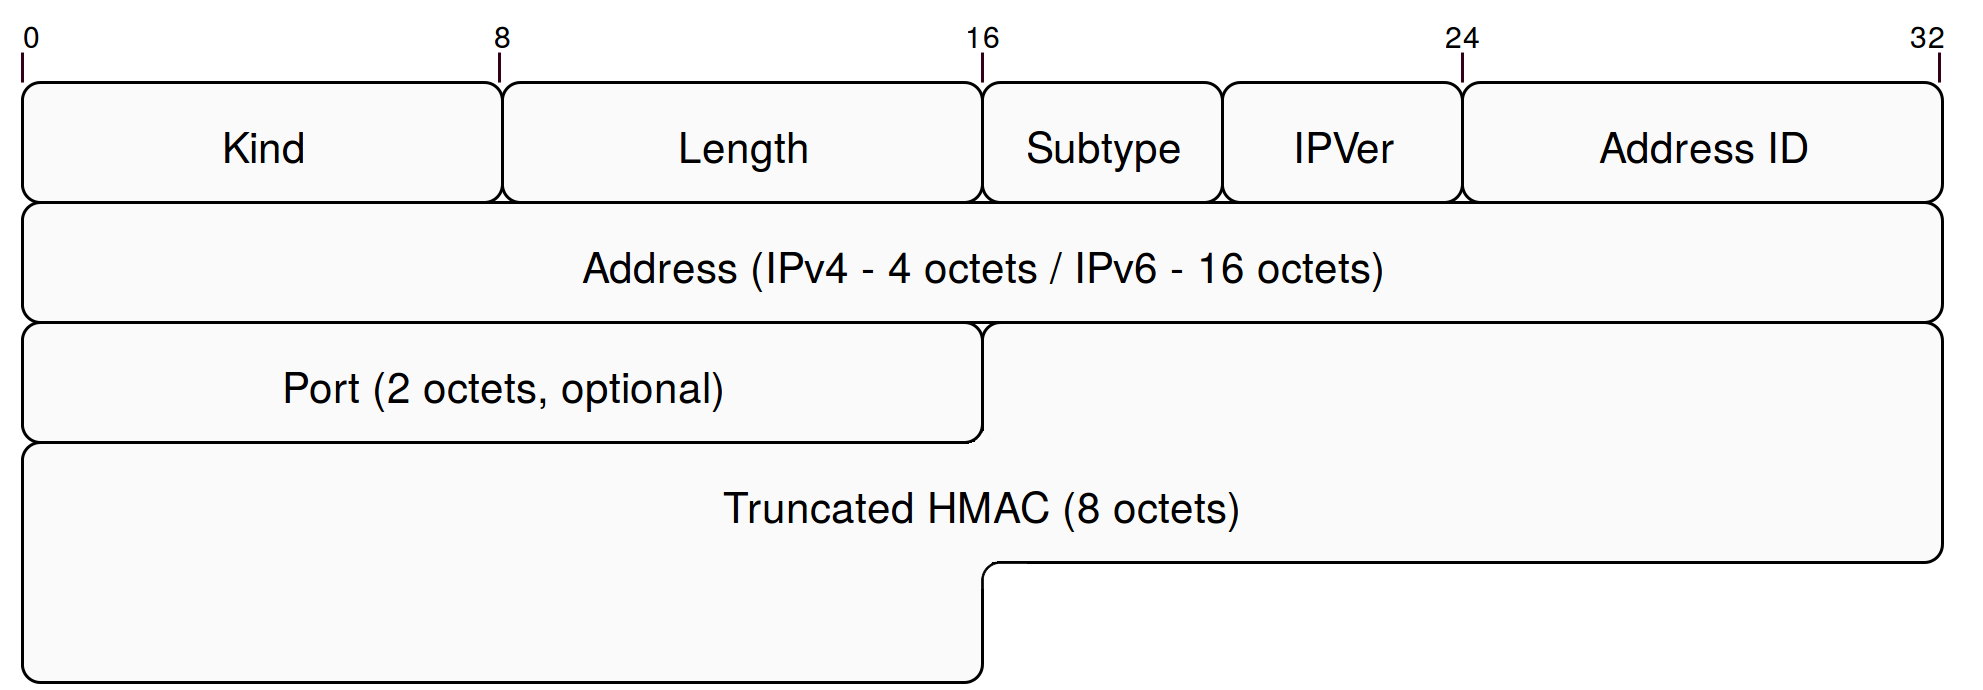
\includegraphics[width=0.85\textwidth]{images/addaddr2}
\caption{ADD\_ADDR2 option \cite{rfc6824bis04})}
\label{fig:addaddr2}
\end{figure}

Such format would require the attacker to know the MPTCP session keys in order to forge a valid ADD\_ADDR2 message, but no keying material or token is exposed with this solution. Albeit, if the attacker is able to eavesdrop the keys during connection initiation it would be possible to exploit the same vulnerability even with the new address format. More experiments about this case are reported in section \ref{exp}. Possible mitigations for such threat concerning keys' eavesdrop are explained in section \ref{keyseav}. The keys' eavesdrop threat is a partial-time on-path eavesdrop, a category that is considered less critical in terms of security concerns. In fact, such keys' eavesdrop procedure in MPTCP has an almost identical counterpart in SCTP, when the SCTP-AUTH extension is used without pre-shared keys \cite{rfc5061}: the same security levels of SCTP would be reached in MPTCP by upgrading ADD\_ADDR to ADD\_ADDR2. Since SCTP is Standard Track, ADD\_ADDR2 is indeed considered a sufficient modification of the MPTCP first design to reach the security levels required for the transition to Standard Track.

\section{Implementing ADD\_ADDR2}
The current MPTCP patch added to the TCP stack in the Linux Kernel currently counts around 12000 lines of code (all the statistics about the code can be found at \url{https://multipath-tcp.org/mptcp\_stats/index.html}). The Linux implementation is considered the reference implementation for MPTCP and it closely follows the RFC specifications. Moreover, a lot of effort has been put into the implementation design in order to make the new protocol acceptable for upstreaming to the official Linux Kernel. For such purpose, it is of paramount importance to keep the added complexity into the TCP stack as low as possible, in order not to jeopardize performance and stability of regular TCP. Nevertheless, high performance is expected for MPTCP. The main architectural concepts related to the control plane of the protocol are now explained, before introducing the modifications related to the new ADD\_ADDR2 format \cite{rfc6824bis04}.

\subsection{MPTCP in Linux}
With MPTCP in the Linux Kernel, three main layers are defined in the networking stack to guarantee multipath management and backward compatibility with regular TCP \cite{BPB11}. The first element is the \textit{master subsocket}, which provides the interface used by the applications to communicate with the TCP stack. The structure of the master subsocket follows the regular TCP standards, in order to maintain backward compatibility towards the application layer: in fact this is the only element used by the Linux Kernel in case of regular TCP connectivity. The second element is called \textit{multipath control block (mpcb)} and it is the main brain of MPTCP, handling MPTCP-specific functionalities: the multipath control block runs the algorithms that determine when to start or stop subflows, which subflow to chose in order to send a particular piece of data over the network and how to reconstruct the original data from the scattered segments coming from different subflows at the receiver. All the reordering algorithms in the multipath control block work at the MPTCP data-level, while the reordering of the data at the single subflows is handled by the underlying regular TCP. The final element of the MPTCP architecture is the set of \textit{slave subsockets}, the actual endpoints for the multiple MPTCP subflows. Such elements are not visible by the application, but they are handled by the multipath control block. The master subsocket and the slave subsockets form the pool of subflows' endpoints used in a MPTCP host. The \textit{mpcb} is referenced in the so called \textit{meta-socket} structure (figure \ref{fig:architecture}).

% Change "multipath control block" with "meta-socket". mpcb is just a component of the meta-socket
\begin{figure}[!htb]
\centering
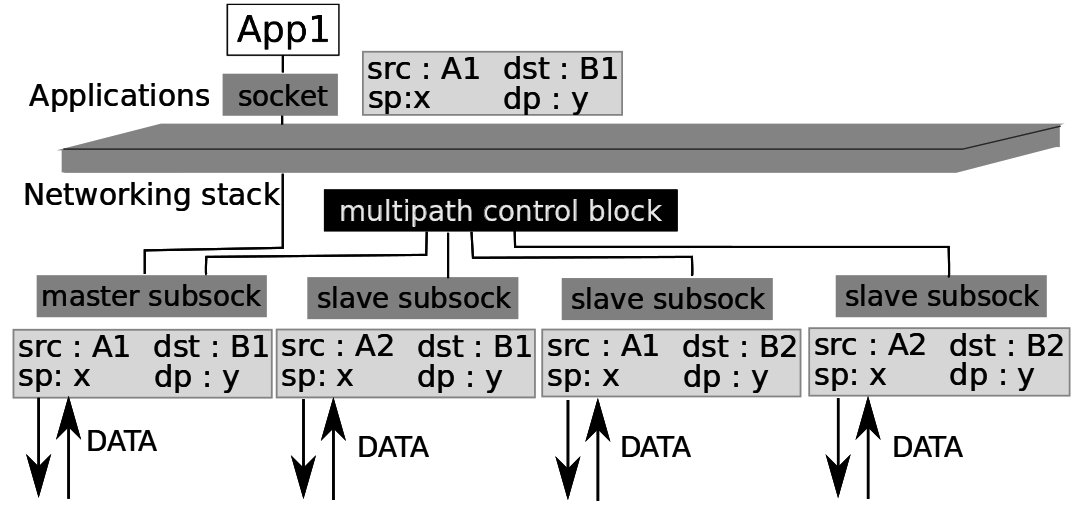
\includegraphics[width=0.9\textwidth]{images/architecture}
\caption{General architecture of MPTCP in the Linux Kernel}
\label{fig:architecture}
\end{figure}
%(reworked from \cite{BPB11})

The actual code implementation related to such architecture is mainly composed of several data structures linked by pointers. In order to maintain the design-goal if minimizing the impact over regular TCP, when a TCP structure would need additional elements to handle MPTCP-related functionalities, the common choice is to define a new MPTCP-specific structure to store those elements. In this way, upon regular TCP operations, there is no increase in memory-footprint and all the standard TCP structures are in place. On top of that, having specific structures for MPTCP code makes it easier to read and understand the MPTCP components inserted into the TCP stack. For example, a fundamental structure in TCP is the \textit{tcp\_sock}, that is used to store the state of a single TCP connection. In MPTCP, additional information for each TCP subflow is needed (for example the address ID associated to each subflow). A new \textit{mptcp\_tcp\_sock} struct has been defined and each subflow contains a pointer to such new structure. The \textit{mptcp\_tcp\_sock} is a separate structure referenced inside \textit{tcp\_sock} in case of MPTCP connectivity.
Also the previously mentioned main architectural element, that is the multipath control block, is implemented in code using a new structure called \textit{mptcp\_cb}.

The allocation policy for all the new MPTCP structures is lazy-allocation, meaning that MPTCP structures are allocated only if it is detected that both hosts support the new protocol. This choice is again related to the main purpose of not affecting regular TCP performances when MPTCP fails during negotiation. A downside of this approach is related to the fact that the TCP stack operations are often executed in a soft-interrupt context, that does not allow functions to sleep in order to wait for available memory: this means that memory allocations in the middle of a connection might fail, forcing a fallback to regular TCP.

The following sections contain an in-depth analysis of the ADD\_ADDR functionality implemented in the Linux Kernel and how this was modified during the development of the new format ADD\_ADDR2. In the following sections, the term \textit{ADD\_ADDR} is used to indicate the old format for the option, \textit{ADD\_ADDR2} is sued for the new format, while \textit{ADD\_ADDR(2)} addresses the option in general terms without referring to a specific version. Moreover, the term \textit{HMAC} is often used to indicate the full \textit{HMAC-SHA1} cryptographic function.

%%%%%%%%
%%%%%%%%
%%%%%%%%
%%%%%%%%
%%%%%%%%
%%%%%%%%

\subsection{The hashing function}
\label{newhash}
The current implementation of MPTCP in the Linux Kernel adopts a specific function for all the HMAC-SHA1 calculations required by the protocol: it is named \textit{mptcp\_hmac\_sha1()} and it is placed inside \textit{net/mptcp/mptcp\_ctrl.c}. Before the introduction of ADD\_ADDR2, only the MP\_JOIN option required such cryptographic functionality, with a fixed scheme regarding the type and length of the key and message used as input for the HMAC algorithm: the key is always the concatenation of the two 64-bit MPTCP keys exchanged via the MP\_CAPABLE option, while the message is always the combination of two random nonces of 32 bits each (as explained in section \ref{controlplane}). For this reason, the \textit{mptcp\_hmac\_sha1()} has been designed to accept such input values with no flexibility on the length and number of the byte strings passed along for the HMAC computation. The old prototype for the function is shown in listing \ref{oldhmac}.

\begin{lstlisting}[language=c, caption=Prototype for the old \textit{mptcp\_hmac\_sha1()} function, label=oldhmac]
void mptcp_hmac_sha1(u8 *key_1, u8 *key_2, u8 *rand_1, u8 *rand_2,
                     u32 *hash_out);
\end{lstlisting}

The old implementation of the function concatenates the first 8 bytes pointed by \textit{key\_1} and \textit{key\_2} to get the 16-bytes key, and it concatenates the first 4 bytes of \textit{rand\_1} and \textit{rand\_2} to originate the 8-bytes message. The \textit{hash\_out} pointers points to the placeholder for the final result of the calculation (figure \ref{fig:hmacapiold}).

\begin{figure}[!htb]
\centering
\includegraphics[width=0.9\textwidth]{images/hmacAPIold}
\caption{Old API for \textit{mptcp\_hmac\_sha1()} \cite{rfc6824bis04}}
\label{fig:hmacapiold}
\end{figure}

With ADD\_ADDR2 the requirements for the HMAC calculation change. The hashing key follows the same configuration of the MP\_JOIN case, while the message is now the concatenation of some of the fields in the ADD\_ADDR2 option, namely the single-byte address ID, the advertised IP address that can be a 4-bytes IPv4 address or a 16-bytes IPv6 address and, if present, the 2-bytes port value. Instead of implementing a separate hashing function for dealing with the ADD\_ADDR2 case,  it was decided to extend \textit{mptcp\_hmac\_sha1()} in order to accept an arbitrary number of messages of arbitrary length (checking that the total length doesn't exceed a certain limit). For what concerns the HMAC key, that part is expected not to change for future usage in MPTCP since it is most likely based on the two MPTCP keys exchanged during the initial handshake. For the message part, the improved function has been developed using the C functionality for variable argument lists based on \textit{va\_list} (listing \ref{newhmac}, line 2). Only the first part of the new hashing function's implementation is changed, since it is the one that handles the input key and message passed as argument. In such first part, shown in listing \ref{newhmac}, the \textit{input} array is prepared for the actual cryptographic functions called in the second part, the latter being omitted in this paper.

\begin{lstlisting}[language=c, caption=Implementation for the new \textit{mptcp\_hmac\_sha1() function (first part)}, label=newhmac]
void mptcp_hmac_sha1(u8 *key_1, u8 *key_2,
                     u32 *hash_out, int arg_num, ...)
{
    u32 workspace[SHA_WORKSPACE_WORDS];
	u8 input[128]; /* 2 512-bit blocks */
	int i;
	int index;
	int length;
	u8 *msg;
	va_list list;

	memset(workspace, 0, sizeof(workspace));

	/* Generate key xored with ipad */
	memset(input, 0x36, 64);
	for (i = 0; i < 8; i++)
		input[i] ^= key_1[i];
	for (i = 0; i < 8; i++)
		input[i + 8] ^= key_2[i];

	va_start(list, arg_num);
	index = 64;
	for (i = 0; i < arg_num; i++) {
		length = va_arg(list, int);
		msg = va_arg(list, u8 *);
		BUG_ON(index + length > 125); /* Message is too long */
		memcpy(&input[index], msg, length);
		index += length;
	}
	va_end(list);

	input[index] = 0x80; /* Padding: First bit after message = 1 */
	memset(&input[index + 1], 0, (126 - index));

	/* Padding: Length of the message = 512 + message length (bits) */
	input[126] = 0x02;
	input[127] = ((index - 64) * 8); /* Message length (bits) */
	...
}
\end{lstlisting}

From line 15 to line 19 it is possible to verify that the 16 bytes' key is properly xored with the first 16 bytes of the \textit{input} array as required for the proper HMAC calculation. From line 23 to line 29 the ``for loop'' scans the function arguments by retrieving two subsequent arguments at a time: the first is an integer representing the length of the currently processed message component, while the second is the pointer to the actual message component. After checking that the total length of the concatenated message components is not too long, the current component is properly parsed into the \textit{input} array, before advancing the index accordingly and starting a new loop's iteration. The last part of the code snippet shows some padding additions required by the hashing function's implementation at later stages.
To sum up, the new API requires to pass along the following set of information (in this order): pointer to the first 8 bytes of the key, pointer to the following 8 bytes of the key, pointer to the 20-byte placeholder where to save the final result of the HMAC calculation, the number of HMAC message's parts that have to be processed and, finally, the pointers to the various components for the final HMAC input message, where each of the pointers to a message components has to be preceded by an integer determining the byte-length of the component itself (figure \ref{fig:hmacAPInew}).

\begin{figure}[!htb]
\centering
\includegraphics[width=0.9\textwidth]{images/hmacAPInew}
\caption{New API for \textit{mptcp\_hmac\_sha1()}}
\label{fig:hmacAPInew}
\end{figure}

A few considerations should be made about the total length of the final HMAC input message. From the code on listing \ref{newhmac} it can be seen that the message shouldn't be longer than 61 bytes: this number comes from the limit value 125 in line 26 minus the initial \textit{index} value of 64 in line 22. The value 64 indicates that only the second half of the \textit{input} array is reserved for the message, being the first part used for the key instead. Regarding the limit value 125, it has been chosen so that, even in the worst case, the first bit after the message can be set to one (actually, the entire byte after the last byte of the message is set to 0x80), keeping the very last two fields in the 128-bytes \textit{input} array reserved for storing the length value composed as the sum of 512 (bits composing the first half of the input array) plus the number of bits composing the actual HMAC message. Such configuration is required by the subsequent cryptographic functions (omitted) to work.
61 bytes for the HMAC message is a very conservative value for the MPTCP case. As of now, the longest possible message to be processed for ADD\_ADDR2 would be of length 19 bytes: 1 byte for the address ID, 16 bytes for the IPv6 address and two more bytes for the port value.
Moreover, it has been decided to introduce a BUG\_ON macro as a check for the message length, so that the whole system would crash in case the message is too long. Even if crashing the whole Kernel in case of a failure in MPTCP might seem a too drastic approach, the reasoning behind it is that such input messages does not depends on any external input: in other words, the number and length of the message components passed to the hashing function are hardcoded inside the Kernel code and they are within the limits, meaning that such BUG\_ON procedure will never be called during normal execution of the current implementation. Only new uses of the hashing function introduced by Kernel developers could introduce a wrong usage of the new API: during the development phase it is reasonable to crash the whole system if something goes wrong, providing all the means for the developers to notice and address the problem.

Extending the hashing function used in MPTCP as just described has been the final solution adopted to implement ADD\_ADDR2. Nevertheless, another important investigation has been performed about an alternative way to achieve HMAC calculation within MPTCP. Such alternative takes into consideration the usage of the Crypto API framework, that is already available in the Linux Kernel. Code re-usability is a fundamental aspect of Kernel development, and the Crypto module offers all the most popular block ciphers and hash functions computations, including the HMAC-SHA1. Such API has been introduced in the Linux Kernel version 2.5.45 \cite{cryptoinkernel}, and it is now considered very stable and optimized for fast performances.
A patch to test the behavior of Crypto APIs in MPTCP has been developed and tested \cite{cryptopatch1} \cite{cryptopatch2}. The \textit{mptcp\_hmac\_sha1()} API would be still extended to achieve better flexibility in managing the input message components, but it would end up being a simple wrapper calling the Crypto API functions, as shown in listing \ref{crypto} (in this case the entire function's implementation is shown).

\begin{lstlisting}[language=c, caption=\textit{mptcp\_hmac\_sha1()} using Linux Kernel Crypto APIs, label=crypto]
void mptcp_hmac_sha1(u8 *key_1, u8 *key_2, u8 *hash_out, int arg_num, ...)
{
	struct mptcp_hmacsha1_pool *sp;
	struct scatterlist sg;
	u8 *key;
	int i;
	int length;
	u8 *msg;
	va_list list;

	sp = mptcp_get_hmacsha1_pool();
	if (!sp)
		goto clear_hmac_noput;
	sp->hmacsha1_desc.flags = 0;
	key = sp->key_placeholder;

	memcpy(&key[0], key_1, 8);
	memcpy(&key[8], key_2, 8);

	if (crypto_hash_setkey(sp->hmacsha1_desc.tfm, (u8 *)key, 16))
		goto clear_hmac;
	if (crypto_hash_init(&sp->hmacsha1_desc))
		goto clear_hmac;

	va_start(list, arg_num);
	for (i = 0; i < (arg_num); i++) {
		length = va_arg(list, int);
		msg = va_arg(list, u8 *);
		sg_init_one(&sg, msg, length);
		if (crypto_hash_update(&sp->hmacsha1_desc, &sg, length))
			goto clear_hmac;
	}
	va_end(list);

	if (crypto_hash_final(&sp->hmacsha1_desc, hash_out))
		goto clear_hmac;
	mptcp_put_hmacsha1_pool();
	return;

clear_hmac:
	mptcp_put_hmacsha1_pool();
clear_hmac_noput:
	memset((u8 *)hash_out, 0, 20);
	return;
}
\end{lstlisting}

Some of the Crypto functions' operations are straightforward: from a high level perspective, \textit{crypto\_hash\_setkey()} sets the HMAC-SHA1 key, \textit{crypto\_hash\_update()} automatically adds component to the HMAC-SHA1 message every time it is called and finally the \textit{crypto\_hash\_final()} computes the HMAC-SHA1 value.
However, there is an important initialization part that is required for proper functioning of such Crypto functions, that is performed at the very beginning of the connection establishment, i.e. in the \textit{tcp\_init\_sock()} function (in \textit{net/ipv4/tcp.c}). The reason why the initialization part is performed at an early stage during connection establishment instead of just before the need to compute the HMAC value is that the Crypto library is not designed to work in an atomic context, since it involves memory allocations with the option GFP\_KERNEL: such option allows the allocation function to sleep and wait for available memory if that is not immediately ready. However, sleeping is not allowed in atomic context execution, which is the context in use when processing the MPTCP options. The function \textit{tcp\_init\_sock()} is not called in an atomic context, and it is a viable option where to insert the allocation function needed for the Crypto library. The Crypto function to allocate the required memory and algorithms is called \textit{crypto\_alloc\_hash()}, and it takes as first argument the kind of hashing algorithm to use, which in MPTCP case is: \textit{"hmac(sha1)"} (listing \ref{cryptoalloc}, line 3).

\begin{lstlisting}[language=c, caption=Initializing the Crypto-API framework in \textit{tcp\_init\_sock()}, label=cryptoalloc]
	struct crypto_hash *hash;

	hash = crypto_alloc_hash("hmac(sha1)", 0, CRYPTO_ALG_ASYNC);
	if (IS_ERR_OR_NULL(hash))
		return;
	per_cpu(mptcp_hmacsha1_pool, cpu).hmacsha1_desc.tfm = hash;
\end{lstlisting}

The \textit{crypto\_hash} structure initialized in the function \textit{tcp\_init\_sock()} is needed by the subsequent Crypto functions present in \textit{mptcp\_hmac\_sha1()}; the structure is saved in the ``per\_cpu'' structure called \textit{mptcp\_hmacsha1\_pool} and it is retrieved from the same structure as shown in line 11 of listing \ref{crypto}. The ``per\_cpu'' usage allows for better performance in a multi-core environment.

This preallocation solution, that calls \textit{crypto\_alloc\_hash()} early on in the MPTCP operational flow, is not enough to guarantee correct functioning of the Crypto framework when the call to \textit{crypto\_hash\_setkey()} is also needed (listing \ref{crypto}, line 20). In fact, by inspecting the function to set the key value in the Crypto framework, it is possible to find cases in which memory allocations of kind GFP\_KERNEL are executed. Since the key has to be set while parsing the ADD\_ADDR(2) option in atomic context, it cannot be guaranteed that sleeping will never be triggered thus causing Kernel crash. To cope with this problem, further investigation has been performed to verify what could cause a GFP\_KERNEL allocation in \textit{crypto\_hash\_setkey()}. If the input key is not aligned in memory as required by the implementation of the hashing algorithm in use with Crypto-API, then another function \cite{shash61} is called for alignment purposes and the alignment process itself can cause sleeping \cite{shash43}. In order to solve also this problem, an additional preallocation has been added right after the  \textit{crypto\_alloc\_hash()}, and shown in listing \ref{keyprealloc}: here, the alignment procedure is performed on the placeholder for the key, whose content might be set later during the MPTCP connection. This preallocation is possible because the length of the key in MPTCP is fixed (\textit{keylen} always has a fixed value of 16).
Also the pointer to the aligned placeholder is added to the \textit{mptcp\_hmacsha1\_pool} struct and retrieved in \textit{mptcp\_hmac\_sha1()} as shown in \ref{crypto}, line 15.

\begin{lstlisting}[language=c, caption=Preallocating an aligned placeholder for the HMAC key, label=keyprealloc]
...
/* Allocating aligned key_placeholder */
alignmask = crypto_hash_alignmask(hash);
absize = keylen + (alignmask & ~(crypto_tfm_ctx_alignment() - 1));
buffer = kmalloc(absize, GFP_KERNEL);
if (!buffer)
	return;
alignbuffer = (u8 *)ALIGN((unsigned long)buffer, alignmask + 1);
per_cpu(mptcp_hmacsha1_pool, cpu).key_placeholder = alignbuffer;
...
\end{lstlisting}

Despite all the precautions adopted in the process, using the Crypto library in the atomic context of the network stack is not a supported out of the box and it is not advisable to deploy such solution. The investigation about the usage of the Crypto-API in the MPTCP implementation stopped at this point, but the entire work and related patches have been made available for future references \cite{cryptopatch1} \cite{cryptopatch2}. If the Crypto framework is updated to work in atomic context, then its usage in MPTCP would be most likely the best option. Another possibility is to study all the possible paths and functions that can be reached by \textit{crypto\_hash\_setkey()} to make sure that all the required memory allocations have been already taken care of before entering the atomic context. For now, the separate function \textit{mptcp\_hmac\_sha1()} made available in MPTCP, whose API has been improved as previously described, is considered the best solution for the cryptographic calculation within the new protocol.

\subsection{Version control}
\label{retrocomp}
ADD\_ADDR2 is substantial modification of an important design aspect of the MPTCP protocol. ADD\_ADDR2 is indeed non interoperable with the current stable implementation of MPTCP version 0, since the augmented length of the option would cause the older network stack to discard the option right away.
ADD\_ADDR2 is considered part of the new MPTCP protocol version number 1, whose implementation has to guarantee backward compatibility. For this purpose, a version control mechanism has to be in place so that hosts can agree on the version to use upon initial handshake and successively operate according to such decision. Since ADD\_ADDR2 is the first step towards the implementation of the new features for MPTCP version 1, no version control mechanism was provided at the beginning of the development phase for ADD\_ADDR2: version 0 was just a fixed value parsed into each MP\_CAPABLE option (option's format is shown in figure \ref{fig:opt_capable}) with no logic attached.

MPTCP version 1 is currently a moving target, so the definitive update for the version is not included inside the patch for ADD\_ADDR2 that is just a part of the future changes introduced with the new version. For this reason, it has been decided to give the system administrator the possibility of dynamically set the MPTCP version via a \textit{sysctl} call, like the following:

\begin{verbatim}
        sysctl -w net.mptcp.mptcp_version=1
\end{verbatim}

It is possible to identify three main phases in the version agreement procedure \cite{rfc6824bis04}:

\begin{enumerate}
  \item The client insert the highest available MPTCP version number it supports into the MP\_CAPABLE option;
  \item When the server gets the first MPTCP packet, it checks the version advertised by the client and answer with the highest version it supports that is less or equal to the client's version;
  \item As a last step, the client receives the answer from the server, and it checks that it is indeed a valid version (i.e. it is no greater than the one the client advertised in the first place); at this point, the client can backtrack to regular TCP if it does not wish to use the requested version.
\end{enumerate}

In developing MPTCP version control mechanism, a problem was related to the fact that the user can change the version in use at any time via a \textit{sysctl} command, meaning that it is possible to change the version in the middle of an MPTCP connection. It is not desirable to change such configuration during the MP\_CAPABLE exchange: it is possible that the first MP\_CAPABLE is retransmitted to the passive opener (following standard TCP retransmission procedures), and the version number inside retransmitted packets must not change from the one used during the very first transmission. For this reason, the configured \textit{sysctl} value is read and initialized for the MPTCP connection at an early stage, namely when \textit{mptcp\_enable\_sock()} (in \textit{net/mptcp/mptcp\_ctrl.c}) is called; there, the value is saved into the newly introduced field \textit{mptcp\_ver} inside the \textit{tcp\_sock} structure (listing \ref{verphase0}, line 6).

\begin{lstlisting}[language=c, caption=MPTCP version agreement (initializing \textit{sysctl} value), label=verphase0]
...
void mptcp_enable_sock(struct sock *sk)
{
	if (!sock_flag(sk, SOCK_MPTCP)) {
		sock_set_flag(sk, SOCK_MPTCP);
		tcp_sk(sk)->mptcp_ver = sysctl_mptcp_version;
	...
\end{lstlisting}

Even if the \textit{sysctl} value is changed by the user after the \textit{mptcp\_enable\_sock()} has been called, the value in \textit{tcp\_sock} for a specific connection is not affected, and that is indeed the value used to create and send the SYN+MP\_CAPABLE option (even in case of retransmissions).
The same initialization procedure is executed when the MP\_CAPABLE packet is received at the server side, meaning that the code for version agreement at the server also retrieves the local MPTCP version via the \textit{tcp\_sock} for the connection (in listing \ref{verphase2}, line 1, \textit{tp} points to \textit{tcp\_sock}).

The function \textit{mptcp\_reqsk\_new\_mptcp()} (in \textit{net/mptcp/mptcp\_ctrl.c}) is called when the message SYN+MP\_CAPABLE is received by the server and the code in listing \ref{verphase2} is executed to set the highest version available that is not greater than the one advertised by the client. The \textit{mopt} pointer points to the structure containing the received MPTCP options from the client, while \textit{mtreq} is a pointer to the \textit{mptcp\_request\_sock} structure, where the final version chosen by the server is saved for now.

\begin{lstlisting}[language=c, caption=MPTCP version agreement (phase 2), label=verphase2]
	if (mopt->mptcp_ver >= tp->mptcp_ver)
		mtreq->mptcp_ver = tp->mptcp_ver;
	else
		mtreq->mptcp_ver = mopt->mptcp_ver;
\end{lstlisting}

The last step of the version agreement involves the final check performed by the client on the version value sent back by the server: it has to be equal or less then the one originally advertised in the first MP\_CAPABLE message. Such check is added to the function \textit{mptcp\_rcv\_synsent\_state\_process()} (in \textit{net/mptcp/mptcp\_input.c}): \textit{tcp\_sk(sk)} is used to obtain the pointer to the \textit{tcp\_sock} structure, where \textit{mptcp\_ver} is retrieved and compared to the server's MPTCP version residing in \textit{mopt\textrightarrow mptcp\_ver} (listing \ref{verphase3}). If the comparison fails, the \textit{fallback} label is hit to trigger the fallback procedure to regular TCP.

\begin{lstlisting}[language=c, caption=MPTCP version agreement (phase 3), label=verphase3]
	if (mopt->mptcp_ver > tcp_sk(sk)->mptcp_ver)
		/* TODO Consider adding new MPTCP_INC_STATS entry */
		goto fallback;
\end{lstlisting}

After these messages have been exchanged, if a proper version has been agreed, both hosts will eventually call \textit{mptcp\_create\_master\_sk()} and in turns \textit{mptcp\_alloc\_mpcb()} with the information about the version, so that it is also saved in the MPTCP control block \textit{mptcp\_cb} for the session. From the multipath control block, the MPTCP version in use can be retrieved to process the ADD\_ADDR(2) option accordingly.

\subsection{Truncated HMAC in ADD\_ADDR}
\label{hmacinaddaddr}
In the two previous sections two new features have been explained: a new API for the cryptographic function used in MPTCP and a fully functioning version control mechanism for the initial handshake in MPTCP. Both these features are used when processing ADD\_ADDR(2), whose functioning now depends on the MPTCP version in use for the session and, in case of ADD\_ADDR2, it also requires a HMAC-SHA1 calculation.
In order to visualize the operational flow regarding ADD\_ADDR(2) in the MPTCP network stack it is possible to inspect figure \ref{fig:addr2stack}, that shows all the main functions and structures mentioned in the following paragraphs. 

\begin{figure}[!htb]
\centering
\includegraphics[width=\textwidth]{images/addr2stack}
\caption{ADD\_ADDR(2) operational flow in the MPTCP network stack}
\label{fig:addr2stack}
\end{figure}

\subsubsection{Redefine ADD\_ADDR packet}
The part of code in the Linux Kernel defining the format of every MPTCP options is contained in the following header file: \textit{include/net/mptcp.h}. For each MPTCP option there is a corresponding data structure in this header file that contains all the fields for the option in the right order, format and alignment. The ADD\_ADDR option is defined in the \textit{mp\_add\_addr} struct. A first step towards achieving a full implementation of ADD\_ADDR2 is indeed to add the truncated HMAC field into the ADD\_ADDR message and place it after the optional port, both in case of IPv4 and IPv6 (listing \ref{mpaddaddr}, lines 18 and 23).

\begin{lstlisting}[language=c, caption=\textit{mp\_add\_addr} struct, label=mpaddaddr]
struct mp_add_addr {
	__u8	kind;
	__u8	len;
#if defined(__LITTLE_ENDIAN_BITFIELD)
	__u8	ipver:4,
		sub:4;
#elif defined(__BIG_ENDIAN_BITFIELD)
	__u8	sub:4,
		ipver:4;
#else
#error	"Adjust your <asm/byteorder.h> defines"
#endif
	__u8	addr_id;
	union {
		struct {
			struct in_addr	addr;
			__be16		port;
			__u8		mac[8];
		} v4;
		struct {
			struct in6_addr	addr;
			__be16		port;
			__u8		mac[8];
		} v6;
	} u;
} __attribute__((__packed__));
\end{lstlisting}

The fields in the data structure resemble the content of ADD\_ADDR as described from a high level prospective in section \ref{mptcpdesign}.
Since the advertised IP address can be a longer IPv6 address or a shorter IPv4 address, a union is used to define the packet structure for both possibilities, while only a single option is selected at runtime.
The HMAC value that is computed using the HMAC-SHA1 algorithm is of 160 bits, but only its ``least significant'' rightmost 64 bits are parsed into the final packet, hence the usage of an array of eight elements of kind \textit{\_\_u8}.
Particular attention is used to correctly pack the structure, in order to avoid additional padding that could be added by the compiler to align the inner fields for performance purposes. Such padding is unwanted in the final packet sent on wire. The \textit{port} field is optional, meaning that additional care has to be taken when creating the struct in order to build the packet: as it will be shown later in this section, when the port value is not available the copying of the HMAC in the struct is performed by using the memory location of the field \textit{mac} reduced by two bytes, so that it will properly be tailed after the advertised IP address (for both IPv4 and IPv6). 

\subsubsection{HMAC calculation at the sender for ADD\_ADDR2}
When the transmission of an ADD\_ADDR2 is triggered, the function \textit{full\_mesh\_addr\_signal()} (in \textit{net/mptcp/mptcp\_fullmesh.c}) is called to prepare all the fields that will be later on parsed into the outgoing packet; at this point, the fields are saved in a \textit{tcp\_out\_options} structure, defined in \textit{include/linux/tcp.h} (only at a later stage the actual bits sent on wire are parsed according to the \textit{mp\_add\_addr} struct previously described). A new \textit{\_\_u64 trunc\_mac} entry has been added to such structure in order to store the new truncated HMAC used in ADD\_ADDR2 (not shown in this paper).
In listing \ref{fullmesh} is reported the added code inside \textit{full\_mesh\_addr\_signal()} that is used to calculate and store the newly introduced HMAC value and save it in \textit{tcp\_out\_options} (whose pointer in the listing is named \textit{opts}). All the code reported so far addresses the IPv4 advertisement, but IPv6 support is provided throughout the entire set of produced patches. It is also possible to notice the conditional statement checking that the MPTCP version in use is indeed 1 or greater (listing \ref{fullmesh}, line 2). The actual hashing function adopted is the new version of \textit{mptcp\_hmac\_sha1()}, whose functioning has been explained in previous sections.

\begin{lstlisting}[language=c, caption=New ADD\_ADDR HMAC calculation (outgoing IPv4 packet), label=fullmesh]
...
if (mpcb->mptcp_ver >= MPTCP_VERSION_1) {
	u8 mptcp_hash_mac[20];
	u8 no_key[8];

	*(u64 *)no_key = 0;
	mptcp_hmac_sha1((u8 *)&mpcb->mptcp_loc_key,
		(u8 *)no_key,
		(u32 *)mptcp_hash_mac, 2,
		1, (u8 *)&mptcp_local->locaddr4[ind].loc4_id,
		4, (u8 *)&opts->add_addr4.addr.s_addr);
	opts->add_addr4.trunc_mac = *(u64 *)mptcp_hash_mac;
}
...
\end{lstlisting}

In the listing above, the key for the HMAC calculation corresponds to the MPTCP key of the sender as defined during the MP\_CAPABLE exchange (\textit{mptcp\_loc\_key}), followed by 8 bytes initialized to 0 (the \textit{no\_key} field). Even if the 8 trailing bytes are not compliant with the specifications considered as reference for this paper \cite{rfc6824bis04}, which only requires the 32-bit key of the sender for the entire key, these trailing 0 bytes are maintained in order not to change the way the hashing function currently manages the keys for the HMAC computation: in fact \textit{mptcp\_hmac\_sha1()} accepts exactly two messages of 8 bytes each and concatenates them to form the final hashing key. This incorrect key is temporarily acceptable since the protocol specifications regarding this aspect change in the more recent drafts \cite{rfc6824bis05}, as reported in section \ref{otherc}, and the eight bytes that are currently set to 0 will contain another key in the newer implementations.
For what regards the message for the HMAC calculation, it is obtained concatenating the address ID (line 10) and the advertised address (line 11). Note that listing \ref{fullmesh} does not include the code for handling the port value in the HMAC. Indeed, port advertisement (which is optional) is not yet part of the current MPTCP implementation in the Linux Kernel. More details about this can be found later in section \ref{portad}.
The HMAC calculation produces 160 bits that are saved in the placeholder called \textit{mptcp\_hash\_mac} (line 3), whose reference is later saved into the new field in \textit{tcp\_out\_options}, in turn referenced by the pointer \textit{opts} (line 12). 

\subsubsection{Writing final ADD\_ADDR(2) option for the on-wire packet}
The pointer \textit{opts} (referencing to the struct \textit{tcp\_out\_options} that has been already prepared in \textit{full\_mesh\_addr\_signal()}) is used in the function \textit{mptcp\_options\_write()} (file \textit{net/mptcp/mptcp\_output.c}), in order to retrieve the saved values and construct the \textit{mp\_add\_addr} data structure (pointer's name: \textit{mpadd}) for the packet sent on wire (listing \ref{mpoutput}).

\begin{lstlisting}[language=c, caption=Building the structure \textit{mp\_add\_addr (mpadd)} for ADD\_ADDR(2) outgoing message, label=mpoutput]
...
mpadd->kind = TCPOPT_MPTCP;
if (opts->add_addr_v4) {
	mpadd->sub = MPTCP_SUB_ADD_ADDR;
	mpadd->ipver = 4;
	mpadd->addr_id = opts->addresses.addr_id;
	mpadd->u.v4.addr = opts->add_addr4.addr;
	if (mpcb->mptcp_ver < MPTCP_VERSION_1) {
		mpadd->len = MPTCP_SUB_LEN_ADD_ADDR4;
		ptr += MPTCP_SUB_LEN_ADD_ADDR4_ALIGN >> 2;
	} else {
		memcpy((char *)mpadd->u.v4.mac - 2,
	           (char *)&opts->add_addr4.trunc_mac, 8);
		mpadd->len = MPTCP_SUB_LEN_ADD_ADDR4_VER1;
		ptr += MPTCP_SUB_LEN_ADD_ADDR4_ALIGN_VER1 >> 2;
	}
}
...
\end{lstlisting}

In \textit{mptcp\_option\_write()}, the MPTCP version in use is again checked to determine if to process the HMAC field in \textit{opts} or not. If the version is 1 or greater, then a \textit{memcpy} of the first 8 bytes of the HMAC value is performed to the location defined by the following pointer (listing \ref{mpoutput}, line 12): \textit{(char *)mpadd\textrightarrow u.v4.mac - 2}; the ``-2'' is used to start the copying right after the advertised address (IPv4 address, in this case), thus skipping the optional port field. It is important to remind that the actual implementation of MPTCP for the Linux Kernel lacks the feature about port advertisement: more precisely, a port is never added to the ADD\_ADDR(2) option, but the code to handle a possible port value upon ADD\_ADDR(2) reception is in place and fully operational. Further considerations on port advertisement capabilities can be found in section \ref{portad}. 
The new ADD\_ADDR2 has different lengths with respect to the previous version, since the 8 bytes truncated HMAC is added. New length values are defined, by adding ``\_VER1'' to the name of the previous definitions: \textit{MPTCP\_SUB\_LEN\_ADD\_ADDR4\_VER1} is 16 (8 in ADD\_ADDR), and \textit{MPTCP\_SUB\_LEN\_ADD\_ADDR6\_VER1} is 28 (20 in ADD\_ADDR). 
At this point, the ADD\_ADDR2 option with the added truncated HMAC field is ready and sent on wire. In the following paragraph it is presented how the option is processed at the receiver, including the HMAC validation.

\subsubsection{Validate ADD\_ADDR(2)'s length at the receiver}
When the ADD\_ADDR(2) message is received by a host, the length of the received option is checked and it has to match with the expected values, according to the type of message (ADD\_ADDR or ADD\_ADDR2). This check is called in the function \textit{mptcp\_parse\_options()} (listing \ref{badsize}).

\begin{lstlisting}[language=c, caption=Check ADD\_ADDR(2) size at the receiver inside \textit{mptcp\_parse\_option()}, label=badsize]
...
if (!tp)
	break;

if (!is_valid_addropt_opsize(tp->mpcb->mptcp_ver,
			     mpadd, opsize)) {
	mptcp_debug("%s: mp_add_addr: bad option size %d\n",
     		    __func__, opsize);
 	break;
...
\end{lstlisting}

An issue encountered at this point of development was that the function just mentioned was initially called with no reference to the multipath control block structure where the version of the current MPTCP session is stored. In other words, the multipath control block structure is available in the current listing through the pointer \textit{tp\textrightarrow mpcb} (listing \ref{badsize}, line 5), but at the beginning of development the \textit{tp} pointer was not available. The MPTCP version is no more passed along in the options following the MP\_CAPABLE exchange, meaning that the value can't be retrieved directly from inspecting the ADD\_ADDR option. A first workaround was to add the version value in the structure containing the received options, named \textit{mptcp\_options\_received}, before passing this structure to the parsing function. In fact, \textit{mptcp\_options\_received} (whose pointer is available in \textit{mptcp\_parse\_option()} but it doesn't appear in the code snippet of listing \ref{badsize}) is created in another portion of code with access to the MPTCP version in use. However, this might be confusing to the developers, since it looks like the MPTCP version value has been indeed present within the options inside the received TCP segment, while it was in reality saved at connection initialization and just copied from the local \textit{mpcb}. The final approach to solve the problem involved slightly more complex changes for the set of function calls related to the parsing of TCP/MPTCP options: as it can be seen in line 5 of listing \ref{badsize}, the \textit{tcp\_sock} (\textit{tp}) structure containing the \textit{mpcb} data for the connection is available inside the final version developed for \textit{mptcp\_parse\_option()}, and the version value \textit{mptcp\_ver} is passed along to the opsize checking function \textit{is\_valid\_addropt\_opsize()}. This required to modify the \textit{tcp\_parse\_options()} function in the TCP stack to pass along the pointer to the \textit{tcp\_sock}, so that it can be retrieved further down within the function calls chain (listing \ref{tcpparse}, last line). Note that the \textit{tp} pointer can be null in certain cases (for example if \textit{tcp\_parse\_options()} is called from \textit{tcp\_timewait\_state\_process()} while the MPTCP session is shutting down), meaning that a null check is needed before calling the validation function (listing \ref{badsize}, line 2): if \textit{tp} is null, it is impossible to retrieve the MPTCP version and the ADD\_ADDR(2) is simply ignored.

\begin{lstlisting}[language=c, caption=New definition for \textit{tcp\_parse\_options}, label=tcpparse]
void tcp_parse_options(const struct sk_buff *skb,
 		       struct tcp_options_received *opt_rx,
 		       struct mptcp_options_received *mopt_rx,
		       int estab, struct tcp_fastopen_cookie *foc);
		       int estab, struct tcp_fastopen_cookie *foc,
		       struct tcp_sock *tp);
\end{lstlisting}

Regarding the \textit{is\_valid\_addropt\_opsize()} function, it has been developed as a separate inline function since the length's check with the additional ADD\_ADDR2 case involves now four possible configurations and it is quite verbose. Such check simply verifies that the length of the received option complies with the specifications according to the MPTCP version in use the the version of the advertised IP address.

\subsubsection{Validate truncated HMAC for ADD\_ADDR2 at the receiver}
After the host that received the ADD\_ADDR(2) packet has verified the correctness of the option's length, the function \textit{mptcp\_handle\_add\_addr()} takes care of verifying the HMAC and triggering the procedures used to add the advertised address, if appropriate. The IPv4 version of the HMAC verification code at the receiver is shown in listing \ref{addaddrinput}, where the HMAC calculated locally is compared with the one received in the ADD\_ADDR2 message with the \textit{memcmp()} in line 8: the ``return'' in line 10 prevents the information from ADD\_ADDR2 to be further processed, if \textit{memcmp()} fails.

\begin{lstlisting}[language=c, caption=New ADD\_ADDR HMAC calculation (incoming IPv4 packet), label=addaddrinput]
...
mptcp_hmac_sha1((u8 *)&mpcb->mptcp_rem_key,
		(u8 *)no_key,
		(u32 *)hash_mac_check, msg_parts,
		1, (u8 *)&mpadd->addr_id,
		4, (u8 *)&mpadd->u.v4.addr.s_addr,
		2, (u8 *)&mpadd->u.v4.port);
if (memcmp(hash_mac_check, recv_hmac, 8) != 0)
	/* ADD_ADDR2 discarded */
	return;
...
\end{lstlisting}

As expected the code inside \textit{mptcp\_handle\_add\_addr()} is similar to the one used at the sender (\ref{fullmesh}), but in this case, in order to computer the same HMAC value, the local key used for HMAC computation is substituted with the remote key (remote from the perspective of the receiver); moreover, for this code that runs at the receiver, the port value is present and processed if detected inside the ADD\_ADDR(2) option, as it is explained in the following section on port advertisement.

\subsection{Port advertisement}
\label{portad}
Port advertisement in ADD\_ADDR(2) is possible according to RFC specifications but it is only partially supported by the current implementation of MPTCP for the Linux Kernel. In fact, the MPTCP in Linux Kernel is currently able to properly adopt port values advertised in the incoming ADD\_ADDR(2) messages, but there is no code that allows to add the port field in the outgoing messages.
Portions of the code used to process incoming ADD\_ADDR(2) messages is now reported in listing \ref{portreceiver} (IPv4 case is shown).

\begin{lstlisting}[language=c, caption=Handling port field in ADD\_ADDR2 at the receiver, label=portreceiver]
...
if (mpadd->ipver == 4) {
    ...
	recv_hmac = (char *)mpadd->u.v4.mac;
	if (mpadd->len == MPTCP_SUB_LEN_ADD_ADDR4_VER1) {
		recv_hmac -= sizeof(mpadd->u.v4.port);
		msg_parts = 2;
	} else if (mpadd->len == MPTCP_SUB_LEN_ADD_ADDR4_VER1 + 2) {
		msg_parts = 3;
	}
	mptcp_hmac_sha1((u8 *)&mpcb->mptcp_rem_key,
	        			(u8 *)no_key,
			      	(u32 *)hash_mac_check, msg_parts,
				    1, (u8 *)&mpadd->addr_id,
				    4, (u8 *)&mpadd->u.v4.addr.s_addr,
				    2, (u8 *)&mpadd->u.v4.port);
	...
	if ((mpcb->mptcp_ver == MPTCP_VERSION_0 &&
	     mpadd->len == MPTCP_SUB_LEN_ADD_ADDR4 + 2) ||
	     (mpcb->mptcp_ver == MPTCP_VERSION_1 &&
	     mpadd->len == MPTCP_SUB_LEN_ADD_ADDR4_VER1 + 2))
		port  = mpadd->u.v4.port;
	...
}
...
\end{lstlisting}

It is possible to notice that the port field is identified by inspecting the actual length of the ADD\_ADDR(2) message according to the MPTCP version in use. If the length of the received ADD\_ADDR2 option is equal to \textit{MPTCP\_SUB\_LEN\_ADD\_ADDR4\_VER1 + 2}, then the port value is present together with the advertised IPv4 address (similar code is in place for the IPv6 case): in this case, the \textit{msg\_parts} is set to 3 in order to include the port in the HMAC calculation performed by the call to \textit{mptcp\_hmac\_sha1()}, (whose API is explained in section \ref{newhash}). A similar length check is performed to save the port value found in the ADD\_ADDR(2) option, if present (line 22).

In the previous section it has been mentioned that the port advertisement is not yet supported at the sender (and that can be checked by inspecting listings \ref{fullmesh} and \ref{mpoutput} for the outgoing packets processing).
However, in order to properly test all the patches developed during the thesis work, port advertisement support has been partially implemented to test this functionality. If the Linux Kernel intends to announce an IP address, the first function taking care of processing the new provided address and preparing all the fields for ADD\_ADDR(2) is the following: \textit{full\_mesh\_addr\_signal()} (in \textit{net/mptcp/mptcp\_fullmesh.c}). There, the fields of interest, including the port in this case, are saved into the \textit{opts} pointer (\textit{tcp\_out\_options} struct) and later retrieved in \textit{mptcp\_options\_write()}. In \textit{mptcp\_options\_write()}, a newly introduced flag bit in \textit{opts} called \textit{add\_addr\_port} would be used to determine if a port value has indeed to be written in the outgoing ADD\_ADDR(2) message. The actual ``write'' function \textit{mptcp\_options\_write()} with port advertisement support would look like the one in listing \ref{outport} (IPv4 case shown). The new code can be compared with listing \ref{mpoutput}, the latter being much simpler without the check of the port value.

\begin{lstlisting}[language=c, caption=Code to build the outgoing ADD\_ADDR(2) packet with added support for the port value, label=outport]
	...
	mpadd->kind = TCPOPT_MPTCP;
	if (opts->add_addr_v4) {
		mpadd->sub = MPTCP_SUB_ADD_ADDR;
		mpadd->ipver = 4;
		mpadd->addr_id = opts->add_addr4.addr_id;
		mpadd->u.v4.addr = opts->add_addr4.addr;
		len_align = MPTCP_SUB_LEN_ADD_ADDR4_ALIGN >> 2;
		if (!opts->add_addr_port) {
			mpadd->len = MPTCP_SUB_LEN_ADD_ADDR4;
			goto no_port_v4;
		}
		mpadd->u.v4.port = opts->add_addr4.port;
		if (mpcb->mptcp_ver < 1) {
			mpadd->len = MPTCP_SUB_LEN_ADD_ADDR4 + 2;
			/* Add padding at the end of option */
			padd_area = (char *)&mpadd->u.v4.port;
			padd_area += sizeof(mpadd->u.v4.port);
			*(padd_area++) = TCPOPT_NOP;
			*(padd_area++) = TCPOPT_NOP;
			/* Adding 4 due to port and two NOP's */
			len_align =
			(MPTCP_SUB_LEN_ADD_ADDR4_ALIGN + 4) >> 2;
			goto next_phase_v4;
		}
		mpadd->len = MPTCP_SUB_LEN_ADD_ADDR4_VER1 + 2;
		memcpy(mpadd->u.v4.mac,
		       (char *)&opts->add_addr4.trunc_mac, 8);
		/* Add padding at the end of option */
		padd_area = (char *)&mpadd->u.v4.mac;
		padd_area += sizeof(mpadd->u.v4.mac);
		*(padd_area++) = TCPOPT_NOP;
		*(padd_area++) = TCPOPT_NOP;
		/* Adding 4 due to port and two NOP's */
		len_align =
		(MPTCP_SUB_LEN_ADD_ADDR4_ALIGN_VER1 + 4) >> 2;
		goto next_phase_v4;
no_port_v4:
		if (mpcb->mptcp_ver < 1)
			goto next_phase_v4;
		mpadd->len = MPTCP_SUB_LEN_ADD_ADDR4_VER1;
		memcpy((char *)mpadd->u.v4.mac - 2,
		       (char *)&opts->add_addr4.trunc_mac, 8);
		len_align = MPTCP_SUB_LEN_ADD_ADDR4_ALIGN_VER1 >> 2;
next_phase_v4:
		ptr += len_align;
	}
	...
\end{lstlisting}

In line 9 it is possible to find the check regarding the presence of a valid port value in \textit{opts\textrightarrow add\_addr4.port}. This code will also add padding in case the port is written into the message. This solution have been adopted during the development work for the thesis in order to test arbitrary ports for both ADD\_ADDR and ADD\_ADDR2. However, the code to handle port writing in the outgoing ADD\_ADDR(2) messages was not eventually merged into the official MPTCP implementation because of the added complexity that is not required at the moment, since no port is ever advertised with the current underlying code for handling path management.

\subsection{IPv6 considerations}
So far, all the code and examples have addressed the advertising of an IPv4 address. IPv6 support was eventually added, and from the code prospective it mainly copies the IPv4 counterpart, with proper modifications related to the new length of the IPv6 address, that is 16 bytes.

The maximum size allowed for the TCP \textit{Options} field is 40 bytes. The ADD\_ADDR2 option would add up to 30 bytes when and IPv6 address is advertised with the port value (32 bytes, if padding is added). Since it is very unlikely that such a long option would fit if other options are already present in the packet, the specifications states that the ADD\_ADDR2 message should be sent in a duplicate ACK, with no other payload or option \cite{rfc6824bis05}.
For example, in the testing scenario adopted for the thesis work, the Timestamp (12 bytes) and DSS (8 bytes) options were always present in the packet together with ADD\_ADDR(2), meaning that the ADD\_ADDR2 with IPv6 was never added to the packets due to the size limits. Indeed, adding the ADD\_ADDR(2) option in the outgoing packets is treated in the current Linux Kernel implementation as a best effort procedure with no available functionality to send the option alone in a duplicate ACK, being the implementation somehow different from what it is suggested in the mentioned RFC document.

Eventually, an intermediate approach has been adopted for the new ADD\_ADDR2 format: only if an IPv6 is advertised, then all the other MPTCP options in the packet are not added (regular TCP options are not affected). This is done in \textit{mptcp\_established\_options()} (in \textit{ net/mptcp/mptcp\_output.c}), where outgoing options are processed in sequence: by checking the version of the advertised IP address, processing the ADD\_ADDR(2) packet information for the outgoing packet, and then reaching ``return'' in the IPv6 case, so that no other options are processed in the function (listing \ref{ipv6}).

\begin{lstlisting}[language=c, caption=Other MPTCP options are not added to the outgoing packet if ADD\_ADDR2 is present (IPv6 case only), label=ipv6]
...
if (unlikely(mpcb->addr_signal) && mpcb->pm_ops->addr_signal) {
	mpcb->pm_ops->addr_signal(sk, size, opts, skb);
	if (opts->add_addr_v6)
		/* Skip subsequent options */
		return;
}
...
\end{lstlisting}


\section{Overall contributions}
\label{otherc}

\subsubsection{MPTCP Linux implementation}
The previous sections described the development process for ADD\_ADDR2 and the related aspects regarding MPTCP version control and the extension of the HMAC-SHA1 function used in MPTCP, including all the considerations related to port advertisement and IPv6.
The overall code has been submitted into four major patches, plus a smaller bug-fix patch:

\begin{itemize}
  \item mptcp: Add MPTCP version control \cite{patch1};
  \item mptcp: Make 'mptcp\_hmac\_sha1' more flexible \cite{patch2};
  \item mptcp: Add ADD\_ADDR2 option \cite{patch3} (bug-fix: \cite{patch5});
  \item mptcp: Add IPv6 support for ADD\_ADDR2 \cite{patch4}.
\end{itemize}

The patches have been merged into the official repository for the Linux Kernel implementation of MPTCP, under the development branch called \textit{mptcp\_trunk}.
The first implementation of ADD\_ADDR2 for MPTCP has been also mentioned in the official MPTCP blog \cite{blog}.

\subsubsection{RFC6824}
As a complementary part of the development process for the MPTCP implementation in the Linux Kernel, there was the effort to improve the official documentation counterpart for the protocol. In particular, a somewhat substantial modification have been proposed regarding the key adopted for the HMAC computation in ADD\_ADDR2. In \rfc{6824bis-04} \cite{rfc6824bis04} it is indicated to use the MPTCP session key of the sender as the only security material, and that is indeed the implementation provided by the current patches, but there is no valid reason not to adopt as the key for the HMAC the sender's key concatenated with the receiver's key. In fact, when an ADD\_ADDR2 is issued the connection is already established, meaning that both hosts know both keys, and concatenating them for the HMAC hashing key improves security overall (an attacker has to know both keys to forge valid HMAC values). Moreover, from an implementation perspective, maintaining the same key configuration used in MP\_JOIN provides code re-usability for the MPTCP hashing function \textit{mptcp\_hmac\_sha1()}.
These reasonings have been pointed out in the official IETF mailing-list and they have been positively reviewed \cite{maillist}: the newer specifications, released in January 2016, modifies the specifications for ADD\_ADDR2 so that both keys are used \cite{rfc6824bis05}. For this reason it was acceptable to keep the \textit{no\_key} value in the code as a temporary (incorrect) implementation of the older specifications, since it will be soon replaced with the key of the receiver (as mentioned in section \ref{hmacinaddaddr}).
In the same email sent to the IETF mailing-list has been pointed out that the port usage for the HMAC message computation is not very clear. In fact, when no port is advertised it should be specified how to handle the HMAC generation, if to avoid the port value at all (as it is the case with the current patches) or to use it anyway with a value of 0. This point has indeed been clarified in the latest RFC draft, opting for the second solution. The RFC section on ADD\_ADDR2 including the new specifications is reported here \cite{rfc6824bis05}:

\begin{verbatim}
   In the same way as for MP_JOIN, the key for the HMAC
   algorithm, in the case of the message transmitted by Host A, will be
   Key-A followed by Key-B, and in the case of Host B, Key-B followed by
   Key-A.  These are the keys that were exchanged in the original
   MP_CAPABLE handshake.  The message for the HMAC is the address ID, IP
   Address, and Port which precede the HMAC in the ADD_ADDR option.  If
   the port is not present in the ADD_ADDR option, the HMAC message will
   nevertheless include two octets of value zero.
\end{verbatim}

The new draft introduces changes that require future modification of the current work presented in the thesis, in order to meet the new specifications.

\subsubsection{RFC7430}
A minor RFC Errata has been sent regarding the document \textit{Analysis of Residuals Threats and Possible Fixes for Multipath TCP (MPTCP)} \cite{rfc7430}), since a wrong classification has been assigned to the SYN/JOIN attack in section 6. Such attack is not a \textit{partial-time on-path eavesdropper} but the type is \textit{partial-time on-path active attacker} \cite{errata}.

\subsubsection{Nimai Scapy tool}
The Scapy tool with MPTCP support (found at \href{https://github.com/nimai/mptcp-scapy}) that has been used to perform all the attacking tests have been slightly modified to make it compatible with the new format for ADD\_ADDR2. In this way it was possible to test the new packet format and verify the correct functioning of the implemented patches (as shown in the following section \ref{exp}, \textit{Experimental evaluation}). It was sufficient to add the new truncated HMAC field in the class definition for the ADD\_ADDR messages, found in \textit{scapy/layers/mptcp.py}, as shown in listing \ref{scapy2} at line 11 (option with no port field) and line 23 (option with the port field).

\begin{lstlisting}[language=Python, caption=Scapy ADD\_ADDR2 class definition, label=scapy2]
...
class MPTCP_AddAddr(MPOption):
    name = "Multipath TCP Add Address"
    subtype = 3
    subsubtype = 8<<4+3
    fields_desc = [ ByteField("length", 16),
                    BitEnumField("subtype", 3, 4, MPTCP_subtypes),
                    BitField("ipver", 4, 4),
                    ByteField("address_id", 0),
                    IPField("adv_addr", "0.0.0.0"),
                    XLongField("snd_mac", 0),] #conditional length

class MPTCP_AddAddrPort(MPOption):
    name = "Multipath TCP Add Address"
    subtype = 3
    subsubtype = 10<<4+3
    fields_desc = [ ByteField("length", 18),
                    BitEnumField("subtype", 3, 4, MPTCP_subtypes),
                    BitField("ipver", 4, 4),
                    ByteField("address_id", 0),
                    IPField("adv_addr", "0.0.0.0"),
                    ShortField("port",0),
                    XLongField("snd_mac", 0),] #conditional length
...
\end{lstlisting}

\subsubsection{Wireshark}
A fundamental tool used for the whole work about testing and developing MPTCP has been the widely popular open-source network packets analyzer Wireshark. The program already provides MPTCP supports, but it couldn't recognize the new truncated HMAC field in the ADD\_ADDR field during the development phase of such new feature. After the MPTCP code has been reviewed and merged, a small patch for Wireshark has been submitted in order to add support for ADD\_ADDR2. This patch allows to show the actual truncated HMAC field when inspecting an ADD\_ADDR2 message, instead of displaying the 8 raw bytes as an unknown component of the packet. Moreover, it allows to filter the capture file based on the HMAC field in ADD\_ADDR2. The patch has been merged into the official Wireshark repository \cite{wireshark}.

\subsubsection{Linux SCTP}
While investigating the usage of Crypto-APIs in MPTCP, it was decided to inspect how the framework is used in similar scenarios in the latest Linux Kernel. The SCTP protocol, already mentioned in the introductory sections for its similarities with MPTCP, does adopt the Crypto library to perform hashing operations that require the \textit{crypto\_hash\_setkey()} \cite{auth751}, in the same atomic context of the MPTCP case. To verify this, Linux Kernel 4.1.0 has been compiled with the option \textit{CONFIG\_DEBUG\_ATOMIC\_SLEEP} enabled and a SCTP connection has been started. The afore-mentioned option provides a warning if a function that might potentially sleep is called inside an atomic section: the SCTP connection triggered such warning. An email has been sent to the official linux-crypto mailing-list for clarifications, and the issue with the current SCTP implementation has been acknowledged \cite{cryptomail}.

\section{Experimental evaluation}
\label{exp}
The first Scapy script developed to exploit the ADD\_ADDR vulnerability and reproduce the hijacking attack in a simulation environment can be considered part of the experimental evaluation for the thesis work. However, this section focuses on the evaluation of the final products of the development process, mainly investigating the security enhancements and related performance implications introduced with the new ADD\_ADDR2 format and the other related patches.
Every single step of the development process has been verified with experimental tests.

\subsubsection{Version control}
The MPTCP version control works independently from the subsequent number of subflows and interfaces configuration at the hosts, so it has been tested in a single network scenario (the ``standard'' one shown in section \ref{envsetup}). All the combinations of version advertisements have been tested to make sure that version 1 is established only if available at both hosts. The \textit{sysctl} value used to set the MPTCP version by the system administrator has been constrained to accept only 0 or 1 values for the time being. Moreover, tests have been setup to make sure that the version chosen for the very first MP\_CAPABLE packet is not changed upon retransmission. As explained in section \ref{retrocomp}, in order to cope with this case the \textit{sysctl} value is read early on during initialization of the session and saved inside the \textit{tcp\_sock} data structure for the whole duration of the MPTCP connection. In order to make sure this solution works as expected, proper \textit{iptables} rules have been set at localhost to drop the SYN/ACK packets from the server UML, thus triggering the SYN retransmission at the end UML:

\begin{verbatim}
	sudo iptables -I FORWARD -p tcp --tcp-flags ALL SYN,ACK -j DROP
\end{verbatim}

During the retransmission time, the \textit{sysctl} command has been called to change the MPTCP version number, and it was indeed verified that such change didn't apply to the retransmitted packets; in fact, the updated MPTCP version number would be adopted only upon the creation of a new MPTCP connection.
Another test related to the MPTCP version control was to establish a communication between two hosts running two different Linux Kernel images, one with the MPTCP version control in place, and the second one with the older code that simply advertises version 0 and does not support ADD\_ADDR2. Interoperability has been confirmed, since the version agreement settles to 0 and the older version of ADD\_ADDR is used by both parties.

\subsubsection{Hashing function}
The modifications to the \textit{mptcp\_hmac\_sha1()} function required a deep understanding and evaluation of the correctness of the values produced by the HMAC-SHA1 algorithm. At first, to make sure that the enhanced version of the function was working as expected, MPTCP sessions have been established with older version of the MPTCP Kernel to verify that the HMAC values were verified properly by both implementations. Later, the \textit{openssl} tool have been used to calculate the HMAC-SHA1 value of any input key and message in hex format, in order to have a reference comparison tool to verify that the operations works as expected, for both the new hashing function and the old one. The \textit{openssl} tool is used with the following command in the terminal, with \textit{hex message} and \textit{hex key} to be replaced with the desired hex values:

\begin{verbatim}
	echo -n ‘<hex message>’ | xxd -r -p | \
	openssl dgst -sha1 -mac HMAC -macopt hexkey:<hex key>
\end{verbatim}

The correct functioning of this command line has been verified by running some test cases \cite{rfc2202} and verifying the output.

The same tool was used to verify the correctness of the values retrieved using the Crypto-APIs in MPTCP. This framework turned out to be incompatible with atomic context executions, meaning that it can't be used safely while processing MPTCP options in the network stack. Nevertheless, an experimental evaluation of such configuration has been carried out, by using a preallocation mechanism to cope with the atomic execution problem (as explained in \ref{newhash}).
A Kernel image has been compiled with the following built-it modules (other dependent Crypto modules are active but not shown in the list):
\begin{itemize}
  \item CONFIG\_CRYPTO=y
  \item CONFIG\_CRYPTO\_HASH=y
  \item CONFIG\_CRYPTO\_HMAC=y
  \item CONFIG\_CRYPTO\_SHA1=y
\end{itemize}
After this, the setup was operational. During the tests, no crashes due to a sleeping function in atomic context were observed when the preallocation technique was in place, since both the \textit{crypto\_alloc\_hash()} and the key placeholder alignment functions are executed out of atomic context. These results are limited to the adopted network scenario and UML configurations. In fact, the key alignment process was never triggered due to the fact that, for the HMAC\_SHA1 algorithm in use for Crypto, the alignment mask is equal to 0 (meaning that no alignment is actually needed). In order to force the execution of the alignment process, custom alignment mask values have been set, demonstrating the correct functioning of the pre-alignment code in listing \ref{keyprealloc}. Nevertheless, such experimental evaluation of the Crypto framework is limited to the described setup, and further investigation is needed to inspect all the possible cases in which a sleeping function can be called within the framework, since this would cause deadlock in certain contexts of execution.

\subsubsection{ADD\_ADDR2 operations}
After having evaluated that both the version control and the extended hashing function work as expected, the next important step regards the tests on the new ADD\_ADDR2 format. The correct functioning of MPTCP with the new option have been verified in different configurations, mainly derived from the combinations of the following parameters:

\begin{itemize}
  \item Number of interfaces at the client and at the server (one or two);
  \item IP version in use (IPv4 or IPv6);
  \item Port advertisement in ADD\_ADDR2 (present or not present).
\end{itemize}

The resulting scenarios from combinations of these parameters have been tested during the development process. For the port advertisement checks, an arbitrary port value was inserted into the packets by using the experimental code as reported in section \ref{portad}.

The IPv4 testing involved two main configurations:
\begin{enumerate}
  \item A configuration identical to the model shown in listing \ref{clientconf} for the case of the setup used in the ADD\_ADDR attack simulation. The client has two interfaces with IPv4 support while the server has a single available interface with IPv4 support;
  \item  A configuration in which the client has one interface while two interfaces are available at the server, using the IPv4 addresses shown in figure \ref{fig:network2}: it is fairly straightforward to modify the \textit{client.sh} and \textit{server.sh} scripts presented in the previous sections in order to attach two taps to the server and only one to the client (the scripts for this case are omitted).
\end{enumerate}

\begin{figure}[!htb]
\centering
\includegraphics[width=\textwidth]{images/Network_Scenario_2}
\caption{Network scenario, client one interface and server two interfaces (IPv4)}
\label{fig:network2}
\end{figure}

In setting the second configuration, not only the taps attached to the virtual machines have to be rearranged, but also the interface configuration within the virtual machines has to be modified to set the proper IP addresses and routing tables. The Ubuntu network configuration file in \textit{/etc/network/interfaces} for the server in this new scenario is reported:

\begin{verbatim}
auto lo
iface lo inet loopback

auto eth0
iface eth0 inet static
        address 10.2.1.2/24
        netmask 255.255.255.0
        gateway 10.2.1.1

auto eth1
iface eth1 inet static
        address 10.2.2.2/24
        netmask 255.255.255.0
        gateway 10.2.2.1
\end{verbatim}

Moreover, proper ip routing configurations have been set to direct the packet flows to the right gateways, as shown in the following extract from \textit{ip route} at the server:

\begin{verbatim}
10.2.1.0/24 dev eth0  proto kernel  scope link  src 10.2.1.2
10.2.2.0/24 dev eth1  proto kernel  scope link  src 10.2.2.2
\end{verbatim}

It is important to note that in the first case where the client has two interfaces, not only it advertises the second one using ADD\_ADDR(2), but it also soon after instantiate the new subflow with the server independently from the server's reaction to the received ADD\_ADDR(2) option: in the Linux Kernel implementation, the server would not start the creation of the subflow anyway since only the client does so. By providing the server with two interfaces instead, as it is the case with the second configuration, it is possible to actually trigger subflow establishment at the client exclusively thanks to the received ADD\_ADDR(2) from the server.

The ADD\_ADDR2 has been tested in these two IPv4 configurations and subflow establishment works properly when the HMAC field in the new option is verified.
The two configurations reported so far were replicated for the IPv6 tests. In this case, slightly different changes were applied to the configuration files and scripts, but the final scenarios are similar to the ones for IPv4, just with the updated IP addresses. The new \textit{client.sh} for the IPv6 scenario in which the client has two interfaces is reported in listing \ref{clientsh6}.

\begin{lstlisting}[language=bash, caption=\textit{client.sh} for IPv6 setup, label=clientsh6]
#!/bin/bash

USER=`whoami`

sudo tunctl -u $USER -t tap0
sudo tunctl -u $USER -t tap1

sudo ifconfig tap0 inet6 add 1000:1:1::1/64 up
sudo ifconfig tap1 inet6 add 1000:1:2::1/64 up

sudo sysctl -w net.ipv6.conf.all.forwarding=1
sudo ip6tables -t nat -A POSTROUTING -s 1000::0/8 ! -d 1000::0/8 -j MASQUERADE

sudo chmod 666 /dev/net/tun

./vmlinux ubda=fs_client mem=256M umid=umlA eth0=tuntap,tap0 eth1=tuntap,tap1

sudo tunctl -d tap0
sudo tunctl -d tap1

sudo ip6tables -t nat -D POSTROUTING -s 1000::0/8 ! -d 1000::0/8 -j MASQUERADE
\end{lstlisting}

%The previous script is associated with the following network configuration inside the client UML machine:

%\begin{verbatim}
%auto lo
%iface lo inet loopback

%auto eth0
%iface eth0 inet6 static
%	address 1000:1:1::2
%	netmask 64
%	gateway 1000:1:1::1
%
%auto eth1
%iface eth1 inet6 static
%	address 1000:1:2::2
%	netmask 64
%	gateway 1000:1:2::1
%\end{verbatim}

Appropriate network interface configurations and route rules have been also set to achieve the desired flow redirection through the appropriate taps. Eventually, the IPv6 scenario involving a client with two interfaces and a server with a single interface, with the IPv6 addresses in use, is represented in figure \ref{fig:netip6_1}:

\begin{figure}[!htb]
\centering
\includegraphics[width=\textwidth]{images/Network_Scenario_6_1}
\caption{Network scenario, client two interfaces and server one interface (IPv6)}
\label{fig:netip6_1}
\end{figure}

Finally, a second setup for IPv6 have been set, involving a client with a single interface and a server with two interfaces. All the implementation details about this scenario are omitted here, since they closely resemble the previous configurations, but the final scenario is shown in figure \ref{fig:netip6_2}.

\begin{figure}[!htb]
\centering
\includegraphics[width=\textwidth]{images/Network_Scenario_6_2}
\caption{Network scenario, client one interface and server two interfaces (IPv6)}
\label{fig:netip6_2}
\end{figure}

All the scenarios, two involving IPv4 and two involving IPv6, were tested to ensure that the new ADD\_ADDR2 format works properly. For each and every scenario, port advertisement has been also tested. All the results were positive, but only the outcome of a single scenario is reported in this paper, in appendix \ref{app:b}. Such appendix shows the capture file of an MPTCP version 1 connection involving the new ADD\_ADDR2 option sent from a server with two IPv6 interfaces to a client with a single IPv6 interface, without port advertisement enabled: it is possible to verify that the new subflow is started with MP\_JOIN from the client after receiving the ADD\_ADDR2 message, and the advertised IP address is correctly used.

\subsubsection{ADD\_ADDR2 and keys' eavesdrop}
After having tested the proper functioning of the new MPTCP implementation, this has been exposed to the very same attacking tool used to exploit the old ADD\_ADDR vulnerability. As expected, when the host using MPTCP version 1 receives the ADD\_ADDR message without the truncated HMAC field, it simply discards such packet and no subflow is originated, thus making the connection hijack impossible.

The same result is achieved by sending an ADD\_ADDR2 packet with random truncated HMAC, thus proving the HMAC verification process works as expected in MPTCP version 1.

As a further evaluation of the new format, a modified version of the attacking script has been developed to eavesdrop the initial MPTCP keys exchanged in the MP\_CAPABLE options, thus being able to calculate the correct HMAC for ADD\_ADDR2 and carrying out the connection's hijack towards the updated MPTCP implementation \cite{add-addr2-eav}. This attack is indeed the combination of ADD\_ADDR attack and keys' eavesdrop attack, both explained in the section about MPTCP security.
It is important to remind that such attack requires the attacker to be a partially on-path eavesdropper to retrieve the above-mentioned keys, which constitutes an important limitation for the vulnerability, that is currently considered acceptable (see section \ref{keyseav}). Nevertheless, it is interesting to show the feasibility of this new kind of attack towards ADD\_ADDR2. The new Scapy attack script, acting in the same network configuration of section \ref{envsetup}, is very similar to the one used for exploiting the old ADD\_ADDR vulnerability with the only additional component capable of sniffing the keys in the SYN/ACK+MP\_CAPABLE option sent by the server to the client and using such keys to compute a valid HMAC field for the forged ADD\_ADDR2 message. The cryptographic function in the Scapy script is shown in listing \ref{pycrypto} and it works for the IPv4 advertisement without the port value: the argument \textit{r1} is the address ID value and the argument \textit{r2} is the IPv4 address, while \textit{k1} and \textit{k2} are the two keys for the MPTCP session eavesdropped from the MP\_CAPABLE messages. The additional truncated HMAC value is added to the forged packet by using the modified Scapy class for ADD\_ADDR2 shown in listing \ref{scapy2}. In this case, as expected, the hijacking attack is proved to be still possible.

\begin{lstlisting}[language=Python, caption=HMAC-SHA1 calculation in Python, label=pycrypto]
...
def genhmac_addaddr2(k1, k2, r1, r2):
    """Returns a HMAC-SHA1 with the concatenation of k1 and k2
    as key and the concatenation of r1 and r2 as message.
    k1, k2 are 64bits integers
    r1, r2 are 8bits and 32bits integers, respectively
    Return a 160bits integer
    """
    import hashlib
    import hmac
    import math

    key = xstr(k1).rjust(8,'\00') + xstr(k2).rjust(8,'\00')
    msg = xstr(r2).rjust(1,'\00') + xstr(r1).rjust(4,'\00')
    ...
    return xlong(hmac.new(key, msg=msg, digestmod=hashlib.sha1).digest())
...
\end{lstlisting}

\subsubsection{ADD\_ADDR(2) flooding}
A final performance evaluation has been executed on the new ADD\_ADDR2 format. The newly introduced HMAC value in the ADD\_ADDR2 packet would trigger cryptographic computations at the receiver. Such computations are highly optimized for fast execution and reduced CPU utilization, but they might represent a problem if triggered at a high rate. For example, by studying the impact of the HMAC calculation for the MPTCP operations, it has been found that this accounts for the 25\% of the overall CPU time spent in generating the SYN/ACK+MP\_JOIN packet \cite{P14}.

The possibility to overload a host's CPU is now enabled with ADD\_ADDR2, where an attacker can forge ADD\_ADDR2 messages with random HMAC and flood the target, so that the latter has to call the \textit{mptcp\_hmac\_sha1()} function repeatedly. Two new Scapy scripts have been developed to perform such flooding with both ADD\_ADDR \cite{add-addr-flood} and ADD\_ADDR2 \cite{add-addr-2-flood} so that it is possible to compare the difference in CPU load when the HMAC calculation is added to the flooding procedure towards the client. The \textit{main()} function of the script for the flooding is reported in listing \ref{flood2}.

\begin{lstlisting}[language=Python, caption=Scapy flooding tool (\textit{main()} function), label=flood2]
def main():
    args = parse_args()

    ADVERTISED_IP = args.advertisedIP
    CLIENT_IP = args.clientIP
    SERVER_IP = args.serverIP
    CLIENT_IF = args.clientIf
    SERVER_IF = args.serverIf

    pktl = sniff(iface=CLIENT_IF, lfilter=lambda p: filter_source(p, CLIENT_IP), count=1)

    # Sending ADD_ADDR flood to client
    addaddrlist = []
    addaddrlist.append(forge_addaddr(ADVERTISED_IP, SERVER_IP, pktl[0][TCP].dport, CLIENT_IP, pktl[0][TCP].sport, (pktl[0][TCP].ack)+SEQUENCE_OFFSET, (pktl[0][TCP].seq)-SEQUENCE_OFFSET))

    print "Preparing"
    for i in range (0, 10000):
        addaddrlist.append(addaddrlist[0].copy())
    start = time.time()
    print "Sending"
    sendpfast(addaddrlist, pps=int(args.floodRate), iface=CLIENT_IF, loop=10000, file_cache=True)
    end = time.time()
    print(end - start)
    return
\end{lstlisting}

The network scenario adopted for this attack is the same of the one used for the ADD\_ADDR attack simulation (section \ref{reprattack}) and the command line used to call the new attack script is almost unchanged as well: the only difference is the additional argument used to define the rate at which Scapy should send the forged ADD\_ADDR(2) packets (\textit{args.floodRate}). A random HMAC value is added to each packet in case of ADD\_ADDR2 (such random value is present in the implementation code for \textit{forge\_addaddr()}, not shown in listing \ref{flood2}).

A separate Python script has been developed together with \textit{gnuplot} in order to track and visualize the CPU usage of the client virtual machine process over time \cite{monitor}. The tool samples the CPU usage percentage for the UML process from the command \textit{top} (launched from localhost) a number of times defined by the user and it calculates the average of such samples. For our tests, 200 samples are retrieved for each calculation, while the virtual machine is flooded with a fixed rate of ADD\_ADDR(2) packets.

The test involved a \textit{netcat} communication between the client and the server, so that the average CPU usage is practically 0\% when no message is being exchanged. Then, the flooding is executed towards the client (through \textit{tap0}) with different sending rates, from 20000 packets per second up to 100000 packets per second. Initially, the tests were performed with a maximum sending rate of around 1000 packets per second, since it appeared to be the highest throughput reachable by Scapy using the function \textit{send()}. For the final experiment, the function \textit{sendpfast()} is used instead: such function adopts \textit{tcpreplay} to drastically increase the sending rate capabilities of Scapy, thus allowing the experiment on ADD\_ADDR(2) flooding.

\begin{figure}[!htb]
\centering
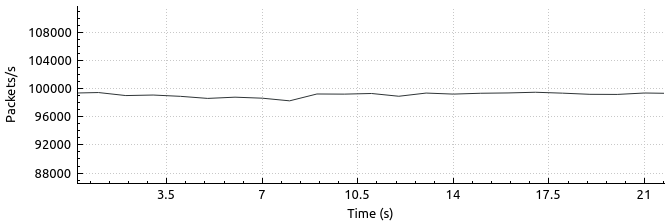
\includegraphics[width=\textwidth]{images/wirethrough}
\caption{Flooding traffic with sending rate set to 100000 packets/sec}
\label{fig:sendgraph}
\end{figure}

In defining the sending rates to be used, it was verified that no packets were dropped by the receiving kernel and that the actual throughput of the flooding tool resembles the value passed as parameter to \textit{tcpreplay}. For these purposes, Wireshark has been used to inspect the actual traffic, and it was possible to verify that Scapy was able to maintain the required sending rate with a good approximation: the results for the most CPU-intensive case, involving 100000 packets per second, show that the actual throughput average is lower than the expected value but always higher than 99000 packets per second (less than 1\% difference). More importantly, the same difference is observed for both ADD\_ADDR and ADD\_ADDR2 packets, meaning that its influence on the comparison between the two formats can be considered very limited. A typical flooding traffic for the simulation is reported in figure \ref{fig:sendgraph}, with a sending rate set to 100000 packets per second. Both ADD\_ADDR and ADD\_ADDR2 flooding have been executed, and each configuration has been run five times for better statistics. The targeted virtual machine (the client UML) was assigned to a single core of the eight Intel Core i7-4770S CPUs (3.10GHz) available inside the physical machine. 256MB was the amount of assigned RAM. The results of such experiment are shown in graph of figure \ref{fig:floodgraph} and in the table \ref{table:floodtable}.

\begin{table}[h!]
\centering
\begin{tabular}{ |p{5cm}|p{1.2cm}|p{1.2cm}|p{1.2cm}|p{1.2cm}|p{1.2cm}|   }
\hline
Flooding rate (pkt/sec) &20k&40k&60k&80k&100k \\
\hline
CPU usage (ADD\_ADDR) & 11,22\% & 22,18\% & 33,00\% & 46,43\% & 55,88\% \\
CPU usage (ADD\_ADDR2) & 12,66\% & 25,03\% & 37,47\% & 52,09\% & 63,38\% \\
Relative increase & 13,41\% & 12,19\% & 13,55\% & 12,86\% & 12,78\% \\
Absolute increase & 1,43\% & 2,85\% & 4,47\% & 5,66\% & 7,49\% \\
\hline
\end{tabular}
\caption{Flooding results}
\label{table:floodtable}
\end{table}

The graph shows how the CPU usage increases almost linearly with respect to the number of received ADD\_ADDR(2) per second. However, for the ADD\_ADDR2 case the CPU usage is sightly higher with the respect to the ADD\_ADDR case, as expected because of the additional HMAC calculation performed for each incoming message. Another element that could contribute to increase the CPU utilization at the receiver is the higher throughput to be handled at the network level due to the additional 8 bytes per packet in case of ADD\_ADDR2. In order to verify the impact of such small difference in the throughput, the following experiment has been executed: an MPTCP version 0 connection has been flooded with ADD\_ADDR2 messages and an MPTCP version 1 connection has been flooded with ADD\_ADDR messages; in both cases the option is not processed and the only CPU usage is exploited to handle the incoming flow of bits at the receiver. In both scenarios the CPU utilizations were practically the same for a constant flooding rate, meaning that the difference observable in graph \ref{fig:floodgraph} is due to the HMAC computations only.

For each tested sending rate, the average CPU usage increases of around 13\% (plus or minus 0,5\%) in case of ADD\_ADDR2 packets: for example, the CPU load for the most CPU-intensive tested scenario, involving 100000 packets per seconds, passes from 55,9\% to 63,4\%, in average.

\begin{figure}[!htb]
\centering
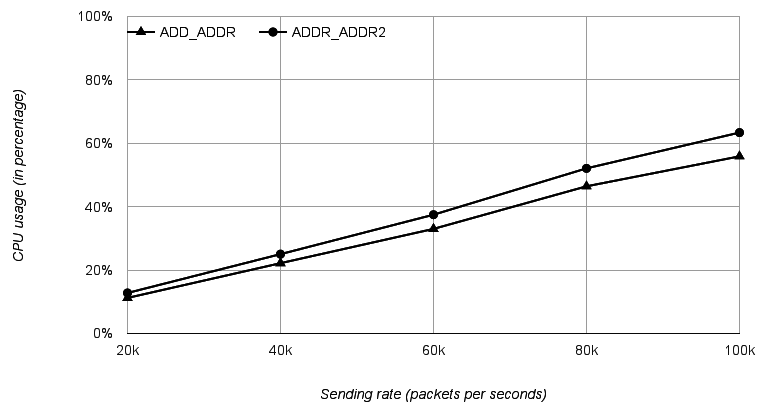
\includegraphics[width=\textwidth]{images/flood}
\caption{Flooding attack for ADD\_ADDR and ADD\_ADDR2 and its impact on targeted host's CPU load}
\label{fig:floodgraph}
\end{figure}

Even if this experiment gives only a rough estimation of the impact brought by the HMAC field in case of flooding attacks, the final data shows a limited increase in CPU usage, not pronounced enough to claim that ADD\_ADDR2 introduces any new attacking vector. Nevertheless, further tests with different operational environments are advised to further investigate the new format's implementation.
